\documentclass[a4paper,9.5pt]{article}
\usepackage[utf8]{inputenc}
\usepackage[spanish,es-tabla]{babel}
\usepackage{geometry}
\geometry{top=0.9cm, bottom=0.9cm, left=1.3cm, right=1.3cm}
\usepackage{xcolor}
\usepackage{hyperref}
\usepackage{enumitem}
\usepackage{titlesec}
\usepackage{fontawesome5}
\usepackage{graphicx}
\usepackage{tikz}
\usepackage[default]{inter}

\definecolor{headerblue}{RGB}{29, 78, 216}
\definecolor{ruleblue}{RGB}{147, 197, 253}
\definecolor{textdark}{RGB}{30, 41, 59}
\definecolor{subtext}{RGB}{71, 85, 105}

\hypersetup{
  colorlinks=true,
  urlcolor=headerblue,
  linkcolor=headerblue
}

\titleformat{\section}{\large\bfseries\color{headerblue}}{}{0em}{}[\vspace{1pt}\color{ruleblue}\titlerule]
\titlespacing*{\section}{0pt}{6pt}{2.5pt}

\setlist[itemize]{label=\textcolor{headerblue}{\small\textbullet}, leftmargin=1.2em, itemsep=1.2pt, topsep=1.2pt, parsep=0pt}

\linespread{1.04}
\pagestyle{empty}

\begin{document}
\color{textdark}

% Header with photo
\noindent
\begin{minipage}[c]{0.78\textwidth}
  {\Huge\bfseries\color{headerblue} Diego De Pablo} \\[3pt]
  {\large\textbf{Software Engineer \textbar\ Full-Stack \& Data Systems}} \\[4pt]
  {\small\color{subtext}
    \href{mailto:depablodiegouma@gmail.com}{\faEnvelope\ depablodiegouma@gmail.com} \quad $\cdot$ \quad
    {\faMapMarker*\ Málaga, España} \\[2.5pt]
    \href{https://linkedin.com/in/diego-de-pablo/}{\faLinkedin\ linkedin.com/in/diego-de-pablo} \quad $\cdot$ \quad
    \href{https://diegodepablo.is-a.dev/}{\faGlobe\ diegodepablo.is-a.dev}
  }
\end{minipage}%
\hfill
\begin{minipage}[c]{0.20\textwidth}
  \centering
  \begin{tikzpicture}
    \begin{scope}
      \clip (0,0) circle (1.15cm);
      \node at (0,0) {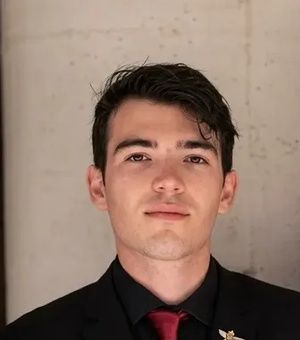
\includegraphics[width=2.4cm]{assets/diego-formal.jpg}};
    \end{scope}
    \draw[ruleblue, line width=1.5pt] (0,0) circle (1.15cm);
  \end{tikzpicture}
\end{minipage}

\vspace{-4pt}

\section*{Perfil Profesional}
Graduado en \textbf{Ingeniería en Bioinformática} y estudiante del \textbf{Máster en Ingeniería Informática}. Especializado en \textbf{desarrollo full-stack}, \textbf{arquitectura cloud nativa} y \textbf{sistemas de datos con IA}. Amplia experiencia construyendo APIs de alto rendimiento con \textbf{FastAPI}, interfaces modernas con \textbf{React/Svelte}, orquestación en \textbf{Kubernetes} e integración de \textbf{agentes LLM} para espacios de datos federados.

\section*{Experiencia Profesional}

\noindent\textbf{Software Engineer, Khaos Research} \hfill {\color{subtext}\textbf{Sept 2025 -- Actualidad}}
\begin{itemize}
  \item Desarrollo end-to-end de aplicaciones full-stack para espacios de datos federados e interoperables (proyecto SEDIA).
  \item Diseño de un buscador semántico con LLM para consultas en lenguaje natural y recomendación de conjuntos de datos.
  \item Creación de servicios modulares de extracción automática de metadatos (+30 formatos) y agentes de workflows.
\end{itemize}

\vspace{2pt}
\noindent\textbf{FullStack Developer, Msurgery} \hfill {\color{subtext}\textbf{Marzo 2025 -- Julio 2025}}
\begin{itemize}
  \item Migración estructural de repositorios centrales de Svelte 4 a Svelte 5, optimizando rendimiento y reactividad.
  \item Implementación de funcionalidades clave para la plataforma SMOTTS y simulación médica mediante gemelos digitales.
  \item Coordinación técnica con stakeholders internacionales y demostración oficial del producto en el Polo Digital.
\end{itemize}

\vspace{2pt}
\noindent\textbf{Ingeniero de software júnior, T\&B Company Group} \hfill {\color{subtext}\textbf{Junio 2021 -- Diciembre 2021}}
\begin{itemize}
  \item Modernización de servicios legados hacia arquitecturas Java y Angular; resolución de incidencias en producción.
  \item Elaboración de especificaciones técnicas y documentación exhaustiva de APIs REST para acelerar la integración.
\end{itemize}

\section*{Proyectos Destacados (Portafolio Interactivo)}

\noindent\textbf{\href{https://diegodepablo.is-a.dev/projects/tfg-patient-monitoring}{\faExternalLink*\ Pulsera IoT de Monitorización de Pacientes (TFG)}} \hfill {\color{subtext}\textit{C++, FreeRTOS, MQTT, Flutter, FastAPI}}
\begin{itemize}
  \item Sistema embebido e infraestructura de telemetría biomédica en tiempo real con detección de anomalías y alertas clínicas.
  \item Reconocido con \textbf{Calificación 10/10 y Mención de Honor}. Enlace al proyecto con arquitectura y demo interactiva.
\end{itemize}

\vspace{2pt}
\noindent\textbf{\href{https://diegodepablo.is-a.dev/projects/kubernetes-platform}{\faExternalLink*\ Laboratorio Kubernetes \& GitOps Cloud-Native}} \hfill {\color{subtext}\textit{K8s, Argo CD, Helm, Envoy, Longhorn}}
\begin{itemize}
  \item Plataforma cloud reproducible en 7 fases: despliegue automatizado con Argo CD, cifrado con Sealed Secrets y almacenamiento distribuido.
\end{itemize}

\vspace{2pt}
\noindent\textbf{\href{https://diegodepablo.is-a.dev/projects/titan-workflow}{\faExternalLink*\ TITAN Workflow Agent}} \hfill {\color{subtext}\textit{FastAPI, LangChain, LLM Agents, Docker}}
\begin{itemize}
  \item Agente autónomo para la planificación y ejecución validada de pipelines bioinformáticos y analítica sobre datos federados.
\end{itemize}

\section*{Formación Académica e Idiomas}

\noindent\textbf{GRADO EN INGENIERÍA EN BIOINFORMÁTICA} \hfill {\color{subtext}Nota media: 7,96/10 \quad \textbf{Sep 2021 -- Jul 2025}}
\begin{itemize}
  \item Matrícula de Honor en \textbf{Fundamentos de Programación}, \textbf{Sistemas Inteligentes} y \textbf{Proyectos de Bioinformática}.
\end{itemize}

\vspace{2pt}
\noindent\textbf{MÁSTER UNIVERSITARIO EN INGENIERÍA INFORMÁTICA} \hfill {\color{subtext}\textbf{2026 -- Actualidad}}

\vspace{2.5pt}
\noindent\textbf{Idiomas:} \textbf{Español} (Nativo) \enskip $\cdot$ \enskip \textbf{Inglés} (B2 / Competencia profesional y técnica completa).

\section*{Competencias Técnicas}

\noindent\textbf{Lenguajes:} Python, TypeScript, JavaScript, SQL, C++, C, C\#, Java, R.\\[1.5pt]
\textbf{Backend \& Cloud:} FastAPI, Node.js, Express, Docker, Kubernetes, Helm, Argo CD, CI/CD, Linux.\\[1.5pt]
\textbf{Frontend:} React, Svelte / SvelteKit, Angular, HTML5, CSS3, Tailwind CSS.\\[1.5pt]
\textbf{Datos e Inteligencia Artificial:} LangChain, OpenAI / Ollama APIs, Polars, Pandas, scikit-learn, PyTorch.

\end{document}
